
\titledquestion{1-Median with Euclidean distance}

% Variante 1

%Die Firma \textit{PowerEngines} hat einen neuartigen Power-Motor entwickelt, und sucht nun nach einem Standort f�r eine neue Produktionsst�tte. Es gilt dabei zu ber�cksichtigen, dass einmal w�chentlich eine Ladung Power-Motoren an 4 verschiedene Automobil-Werke ausgeliefert werden muss. Die 4 Werke haben die Koordinaten (18, 2), (4, 0), (6, 20) und (12, 18). Die Kosten f�r den Transport einer Ladung belaufen sich auf \EUR 6, \EUR 2, \EUR 7 bzw. \EUR 4 pro Kilometer. Die Entfernung wird mit der Luftlinien-Metrik gemessen.
%
%\begin{enumerate}
%	\item Finden Sie einen optimalen Standort f�r die neue Produktionsst�tte der Firma, welche die Summe der Kosten f�r die Auslieferungen minimiert. Wie hoch sind die w�chentlichen Gesamtkosten? L�sen Sie das Problem mit Hilfe des Miehle-Verfahrens in MS Excel und starten Sie im Koordinatenursprung $(x^0,y^0)=(0,0)$! W�hlen Sie als Abbruchkriterium $ \left\|(x^{t},y^{t})-(x^{t+1},y^{t+1})\right\|_{p=2} :=\delta < 0,005$.
%	
%	\begin{solution}
%		
%		\uline{Gegeben:}	
%		\begin{itemize}
%			\item Kundenstandorte: (18,2),(4,0), (6,20), (12,18)
%			\item Gewichte: 6, 2, 7, 4
%			\item Startstandort: $\left(x^0,y^0\right)=\left(0,0\right)$
%			\item Abbruchkriterium: $\left\|\left(x^t,y^t\right)-\left(x^{t+1},y^{t+1}\right)\right\|_{p=2}<0,005$
%		\end{itemize}	
%		
%		\uline{Rechnung:} Siehe Excel-Datei. (Mit $\epsilon=0$)
%		
%		\uline{Ergebnis:}
%		$x^{13}=10,093$, $y^{13}=16,430$\\
%		Die w�chentlichen Gesamtkosten belaufen sich auf 181,67.
%		
%		
%	\end{solution}
%	\item Stellen Sie graphisch dar, wie sich die Koordinaten der Produktionsst�tte von Iteration zu Iteration ver�ndert haben. Lassen Sie auch die Automobilwerke in Ihrer Graphik anzeigen.
%	\begin{solution}
%		\begin{center}
%			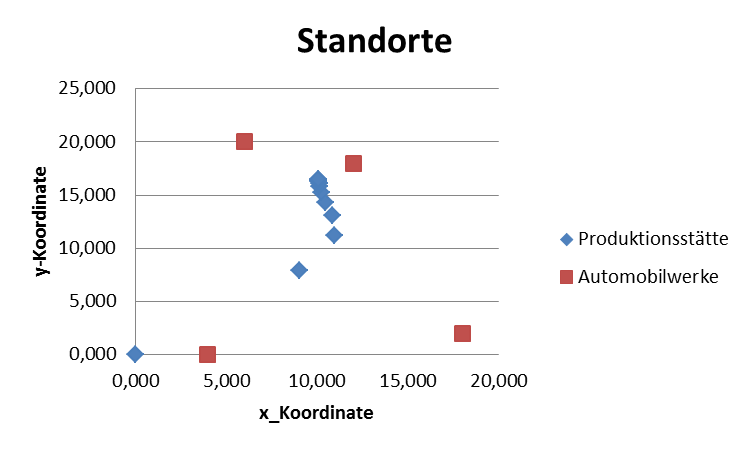
\includegraphics[scale=1.0]{Uebungen/figures/Standorte}
%		\end{center}
%	\end{solution}

% Neue Variante

The company \textit{Cleverfox} plans to open a new manufacturing facility. They want to deliver to all 5 of their customers, once a day, directly from its location. The customers are located at the coordinates (18,5), (5,0), (6,14), (8,8) and (12,18) with respective transportation costs of \EUR 3, \EUR 6, \EUR 2, \EUR 4 and \EUR 8 per kilometer. The OR staff member in the company has measured the distance using the Euclidean distance metric and asked you to determine the optimal location with the help of the Miehle method.

\begin{enumerate}
	\item Find an optimal location for the company's new manufacturing facility that minimizes the total transportation cost. What is the total weekly cost? Solve the problem using the Miehle method in MS Excel, using the origin $(x^0,y^0)=(0,0)$ for the initial iteration! Choose $ \left\|(x^{t},y^{t})-(x^{t+1},y^{t+1})\right\|_{p=2} :=\delta < 0.001$ as the termination criterion.

\begin{solution}

\uline{Input/Given:}	
		\begin{itemize}
			\item Customer locations: (18,5), (5,0), (6,14), (8,8), (12,18)
			\item Weights: 3, 6, 2, 4, 8
			\item Start location: $\left(x^0,y^0\right)=\left(0,0\right)$
			\item Termination criterion: $\left\|\left(x^t,y^t\right)-\left(x^{t+1},y^{t+1}\right)\right\|_{p=2}<0.001$
		\end{itemize}	

\uline{Calculation:} See Excel file. (With $\delta<0.001$)

\uline{Results:}	

	$x^{44}=8.217$, $y^{13}=8.215$\\
	The total weekly transportation cost is $7*95.23 = $\EUR$181.37 $.
	
	
\end{solution}
\item Graphically show how the optimal coordinates of the manufacturing facility change from iteration to iteration. Also display the customer location in your graph.
\begin{solution}
\begin{center}
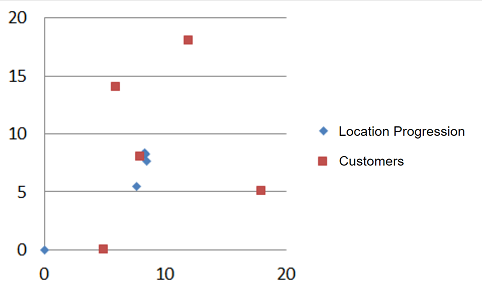
\includegraphics[scale=1.0]{Uebungen/figures/Miehle_Standort_Var2_eV}
\end{center}
\end{solution}

\end{enumerate}
